\section{Collaboration Projects}

Artificial intelligence and machine learning (AI/ML) are utilized across various components of the CLAS12 experiment, including online data monitoring, offline reconstruction, data analysis, and enhanced particle identification. Their integration into the reconstruction process has led to a substantial improvement in the experiments' statistical precision.

\subsection{AI/ML in CLAS12 tracking}

CLAS12 tracking algorithms employ AI techniques to enhance track reconstruction. A sequence of neural networks operates in concert to maximize efficiency. Initially, a Convolutional Autoencoder is applied to denoise raw signals from the Drift Chambers (DC). Subsequently, a Multi-Layer Perceptron (MLP) connects clusters across the six DC superlayers to identify track candidates. To address inefficiencies such as missing segments in one or more superlayers, a secondary autoencoder is used to recover incomplete tracks. The incorporation of AI into CLAS12 reconstruction has led to a significant increase in tracking efficiency (approximately $20\%$ at a 50 nA electron beam on a hydrogen target), resulting in an estimated $60\%$ gain in collected statistics for three-particle final state reactions.

\begin{figure}[h!]
\centering
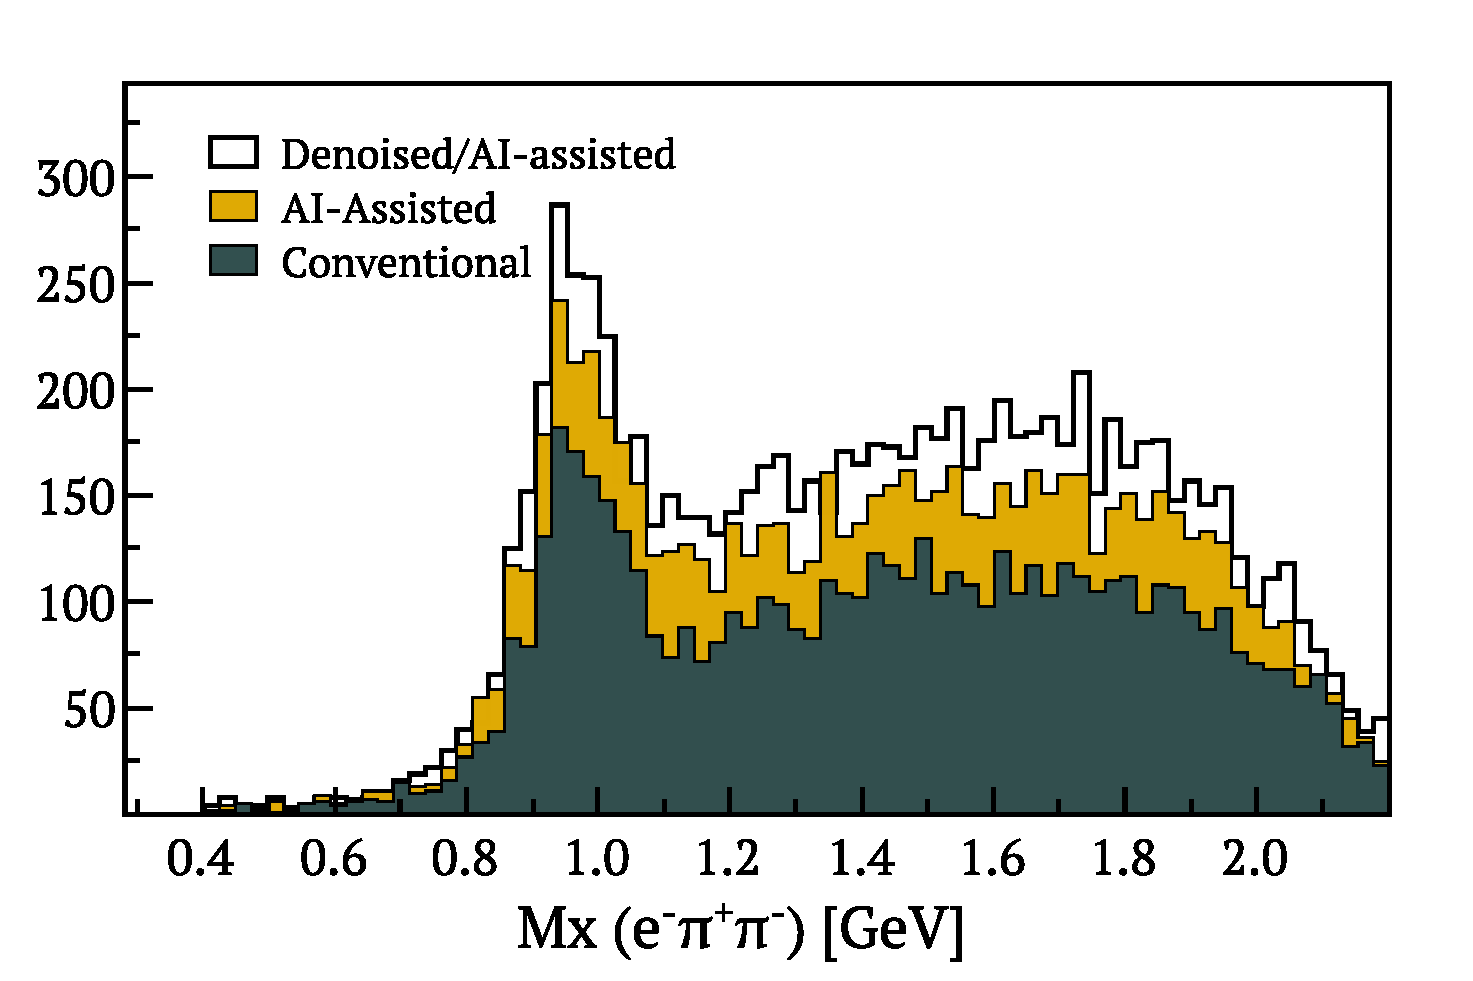
\includegraphics[width=0.42\columnwidth]{images/projects/figure_denoise_mxp.pdf}
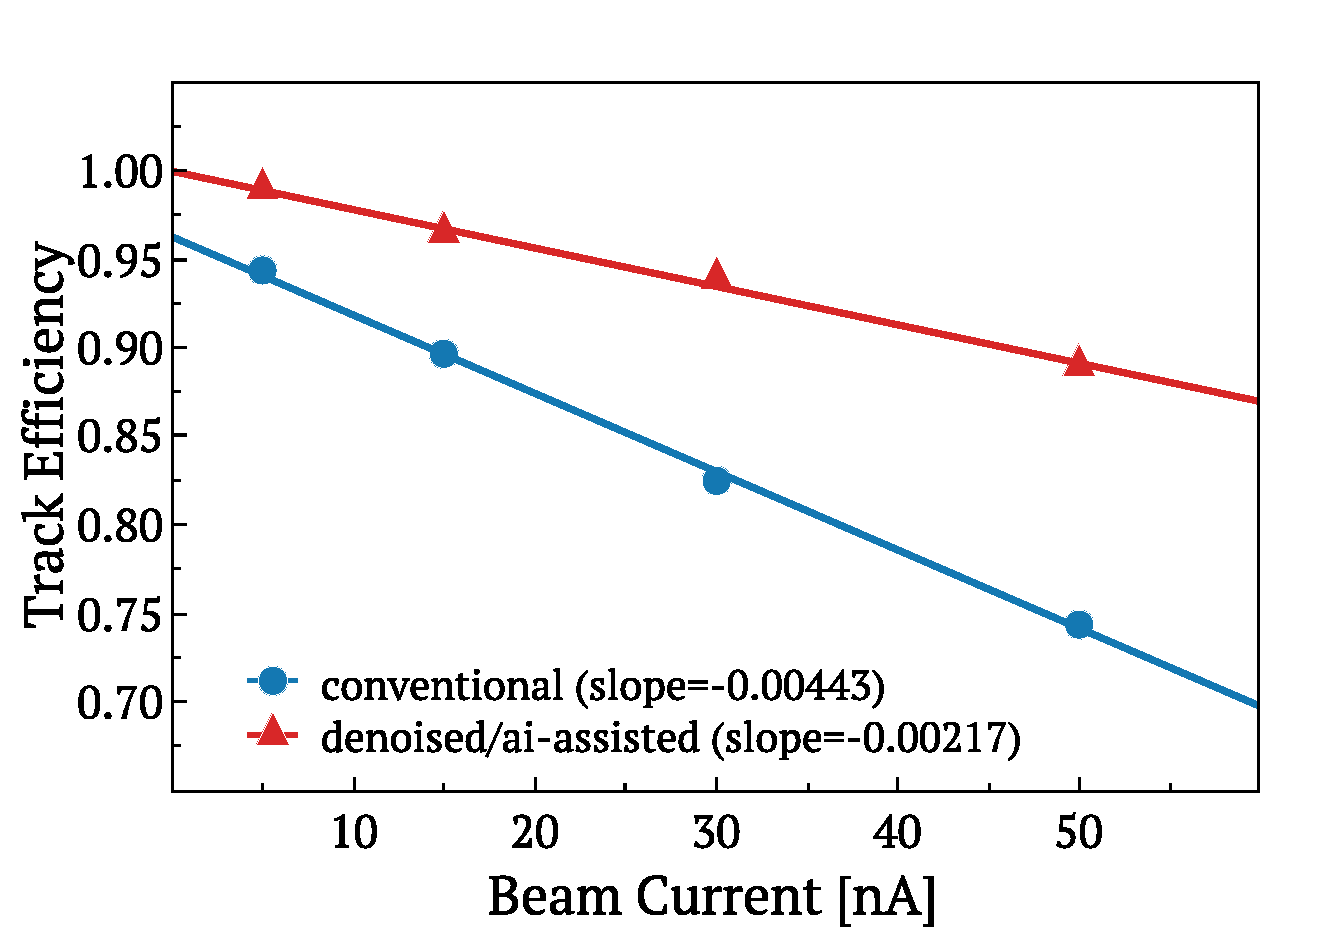
\includegraphics[width=0.42\columnwidth]{images/projects/luminosity_scan.pdf}
\caption{ } 
\label{fig:ai_results}
\end{figure}

Figure~\ref{fig:ai_results} (left) presents the statistical gain for the reaction $H(e) \rightarrow e^\prime\pi^+\pi^-X$, where the missing mass distribution of the detected particles highlights the missing proton. Figure~\ref{fig:ai_results} (right) shows the track reconstruction efficiency as a function of luminosity (beam current), comparing conventional tracking with AI-augmented tracking. The enhanced efficiency achieved through AI integration enables experiments to operate at higher luminosities while maintaining robust track finding performance. AI-augmented track finding has been integrated into the standard data processing workflow and is currently employed in the processing of experimental data.

\subsection{Online Reconstruction in CLAS12}

